\documentclass{article}
% NeurIPS 2026 style files are not published yet (media.neurips.cc .../NeurIPS2026/Styles.zip
% returns 404 as of 2026-07-26); this is the 2025 style, which is the current one. Swap in
% neurips_2026.sty when it appears -- the geometry is what sets the page count.
% Anonymous submission: no [final], no [preprint].
\usepackage{neurips_2025}
\usepackage{graphicx,amsmath,amssymb,booktabs,hyperref,xcolor}
\usepackage[T1]{fontenc}
\graphicspath{{../fig/}}
\hypersetup{colorlinks=true,linkcolor=blue!50!black,citecolor=blue!50!black,urlcolor=blue!50!black}
\newcommand{\dn}{\ensuremath{D_{\mathrm{norm}}}}
\newcommand{\dz}{\ensuremath{D_0}}
\newcommand{\lca}{\ensuremath{\lambda_{\mathrm{ca}}}}
\title{A Validated Black-Box Instrument for Language-Model Dynamics:\\
Reproducing Known Metrics with a Token-Lattice Cellular Automaton}

\begin{document}
\maketitle

\begin{abstract}
We turn a language model into a \emph{cellular automaton over token space}---a ring of token
cells resampled in place by the model's own windowed conditional $p_r(x_i\mid x_{i\pm r})$,
probed by common-random-number (CRN) damage spreading---and develop it into a \emph{validated}
measurement instrument. The organizing principle is \textbf{validation by reproduction}: before
measuring a language model we recover metrics whose values are already known. On the
Domany--Kinzel stochastic automaton, where the damage field is provably the automaton itself,
an independent prediction matches ours \textbf{bit-exactly}---zero mismatching cells over
$4096\times1500$ updates, with a nonzero off-line control---calibrating the apparatus with no
error bar attached; it also separates elementary CA rules by whether damage survives
($d{=}3.0$) and recovers known Markov transition matrices. Applied across
Pythia-410m training checkpoints, it detects a \textbf{developmental transition}: the
token-space Lyapunov exponent goes from seeds disagreeing about its \emph{sign} to
\textbf{every one of 48 post-transition runs being positive}, at two lattice sizes (all four
members of a pre-registered family survive Benjamini--Hochberg correction; $d{=}1.59$ and
$1.76$ against the pre-registered baseline), with seed-to-seed variance collapsing
$\sim\!3\times$. We then \emph{delimit} the instrument, which
is the result we consider most useful: real autoregressive generation absorbs \emph{no}
injected token error ($P_{\text{persist}}{=}1.000$ on three models), because free generation
never resamples a token. These quantities therefore characterise an iterated-resampling
construction, not deployed decoding---a boundary we draw rather than leave to a reader.
\end{abstract}

\section{Introduction}
Language models are evaluated almost entirely as functions: given a context, how good is the
next-token distribution? But a masked or autoregressive conditional also \emph{defines a
dynamics}---iterate it in place over a lattice of tokens and one obtains a stochastic cellular
automaton whose rule is the model. Iterated-map views of LLMs have appeared qualitatively
\citep{logos_ca,telephone,paraphrase2cycle} and as mixing-time studies of masked-LM Glauber
dynamics \citep{glauber_mlm}; the phenomena a CA vocabulary names---damage spreading, light
cones, Lyapunov exponents, attractor censuses \citep{hanson1997computational}---are decades
old. What has been missing is not a phenomenon but a \emph{measurement instrument whose
readings can be trusted}.

Our organizing principle is therefore \textbf{validation by reproduction}
(\S\ref{sec:validation}): before turning the apparatus on a language model, we require it to
recover values that are independently known. This is not a formality. Building the ladder
forced us to retract several of our own earlier claims, and the strongest rung is one where
agreement is \emph{exact} rather than fitted, so it cannot be passed by a plausible-looking
estimator. Only then do we report what the instrument measures on trained LMs
(\S\ref{sec:dev}, \S\ref{sec:other}), and---equally---where its readings provably stop
applying (\S\ref{sec:realgen}, \S\ref{sec:crosslevel}).

A deliberate choice runs through the paper: we use only \emph{simple, mature} primitives---
single-site damage spreading, the damage-spreading Lyapunov exponent \citep{bagnoli1992damage},
the light cone \citep{lieb1972finite}, the attractor census \citep{hanson1997computational}---
rather than bespoke machinery. Their value is that they are \emph{understood}: their behaviour
on known systems is a fixed benchmark, which is what makes reproduction a real test. The
criticality and edge-of-chaos ideas the results touch are old
\citep{langton1990computation,bertschinger2004real,edgeofchaos2024}; our contribution is a
calibrated black-box \emph{measurement} of them, and an explicit statement of its limits.

\section{The instrument}\label{sec:instrument}
\textbf{Rule.} A window of $w=2r{+}1$ tokens with the centre masked is fed to a masked LM; the
tempered centre distribution is the kernel $p_r(x_i\mid x_{i\pm r})$. For an autoregressive
model the window is the $r$ cells to the left and the rule is the next-token
distribution---an order-$r$ causal kernel. \textbf{Automaton.} $N$ ring cells, async
random-order single-site Glauber (synchronous updates manufacture period-2 blinkers and are
only an apparatus arm); special tokens forbidden as emissions. \textbf{CRN coupling.} Twin
lattices sharing initial state, update order, and the uniform stream driving inverse-CDF
sampling differ only in the factor under test, so the \emph{null} arm must diverge by exactly
zero. It does, on every backend---this is asserted in the test suite, not assumed, because
every damage number depends on it.

\textbf{Two confounds shape every metric.} \emph{Repetition}: a lattice looping one corpus
$n$-gram scores high overlap for free, so structure uses a repetition-robust variant.
\emph{Diversity}: a degenerate low-entropy lattice snaps a perturbation back trivially---low
damage for the wrong reason---so damage $D$ is normalized by the model's own diversity floor
\dz{} (the asymptotic drift of twins under \emph{independent} noise with no flip), giving
$\dn=D/\dz$. A free control disciplines our language throughout: the temperature ``phase
transition'' is, on a finite-size scan, a \emph{crossover}
($\chi_{\mathrm{peak}}\propto1/N$), not a true transition.

\section{Validation: reproducing known metrics}\label{sec:validation}
We check the apparatus against systems where the answer is known, and are explicit about which
properties each rung does and does not exercise (Fig.~\ref{fig:ladder}). The ladder is ordered
by how much of the instrument's regime the rung shares: smooth-limit arithmetic first, then
\emph{discrete} state with a finite perturbation---the regime the token instrument occupies.

\textbf{(1--2) Smooth-limit unit tests, labelled as such.} A renormalized tangent estimator
recovers the logistic map's analytic exponent to machine precision, and a coupled-map lattice
matches an exact Benettin/Jacobian reference to $1.1\times10^{-3}$. Neither is evidence about
damage spreading: the twin is re-anchored to the reference orbit each step, so the estimator
\emph{is} a finite-difference evaluation of the derivative it is compared against (an
$\epsilon$-sweep confirms error $O(\epsilon)$), and \textbf{a token flip is $O(1)$ in a
discrete alphabet---there is no $\epsilon\to0$ limit in token space}.

\textbf{(3) Elementary CA: a coarse split, decisively.} Driving the identical protocol with 19
rules of \emph{known} class (12 seeds, rule as the unit of analysis) separates rules whose
damage \emph{survives} from those whose damage \emph{dies}. The discriminating quantity is the
\textbf{ignition probability}, not $\lambda$: damage in a discrete CA is bimodal, so a
$\lambda$ averaged over ignited and extinguished runs measures the mixture. It is also the
physically correct object, being the order parameter of the directed-percolation class
\citep{grassberger1995}. Ordered rules sit at $0.046$ (CI $[0.000,0.102]$) against $0.668$
(edge) and $0.682$ (chaotic): \textbf{ordered vs.\ rest $p{=}0.0$, $d{=}3.03$}. The finer
three-class ordering does \emph{not} survive ($p{=}0.470$), so we claim only the coarse split.
We report this rather than the group-mean $\lambda$ ordering we first computed, for two
reasons: that ordering was not significant edge-vs-chaotic, and its ordered-group mean is not
a measurement---five of seven ordered rules return exactly $-0.4\ln10$ with a zero-width
interval, the constant a log-linear fit yields when damage dies immediately and the cone hits
the estimator's numerical floor.

\textbf{(4) Domany--Kinzel: an \emph{exact} check on the damage machinery.} The DK automaton
\citep{domany1984} is the only rung that is stochastic \emph{and} discrete---the instrument's
own regime. On its $p_2{=}0$ line the damage field between two commonly-driven replicas is
provably \emph{itself} a DK automaton at the same $p_1$ \citep{kohring1992}: with
$s'_i=(s_{i-1}\oplus s_{i+1})\,\theta(p_1-z_i)$, sharing $z_i$ gives
$d'_i=(d_{i-1}\oplus d_{i+1})\,\theta(p_1-z_i)$. We therefore predict the damage trajectory
with an independent simulator and demand \emph{bit-identity}: across $p_1\in\{0.2,\dots,1.0\}$
on a ring of $4096$ over $1500$ steps, \textbf{zero mismatching cells}, with $16$ in an
off-line control at $(0.6,0.5)$ where the mapping must break. This runs through the same
simulation loop that produces every language-model number below, so the window indexing, the
shared-uniform consumption order, the sampling and the update schedule are verified with no
error bar attached. A second closed form rides inside the same run: at $p_1{=}1$ the update is
deterministic $\oplus$ (Rule 90), so the damage field must hold exactly
$2^{\mathrm{popcount}(t)}$ live cells---at $t{=}1500$, $128/4096=0.03125$, which is what we
obtain. Critical points are a weaker, $\sim\!1\%$ check: $p_c{=}0.7065$ on the site-DP line
(published $0.705489(4)$) and $0.8092$ on $p_2{=}0$, where the published value is itself
disputed ($0.801(2)$ \citep{zebende1994} vs.\ $0.8087(5)$ \citep{hinrichsen1997}) and our
accuracy cannot separate them; we report both and claim neither.

\textbf{(5) Synthetic Markov sources.} The attractor census, run on tiny models trained on
three sources with known sparse matrices, recovers each model's own matrix (row
total-variation $0.22$) and not the others (cross $0.95$; random baseline $0.91$).

Rungs (3)--(5) share the instrument's regime and are what license its use on language models;
(4) is the only one on which agreement is exact rather than fitted.

\begin{figure}[t]\centering
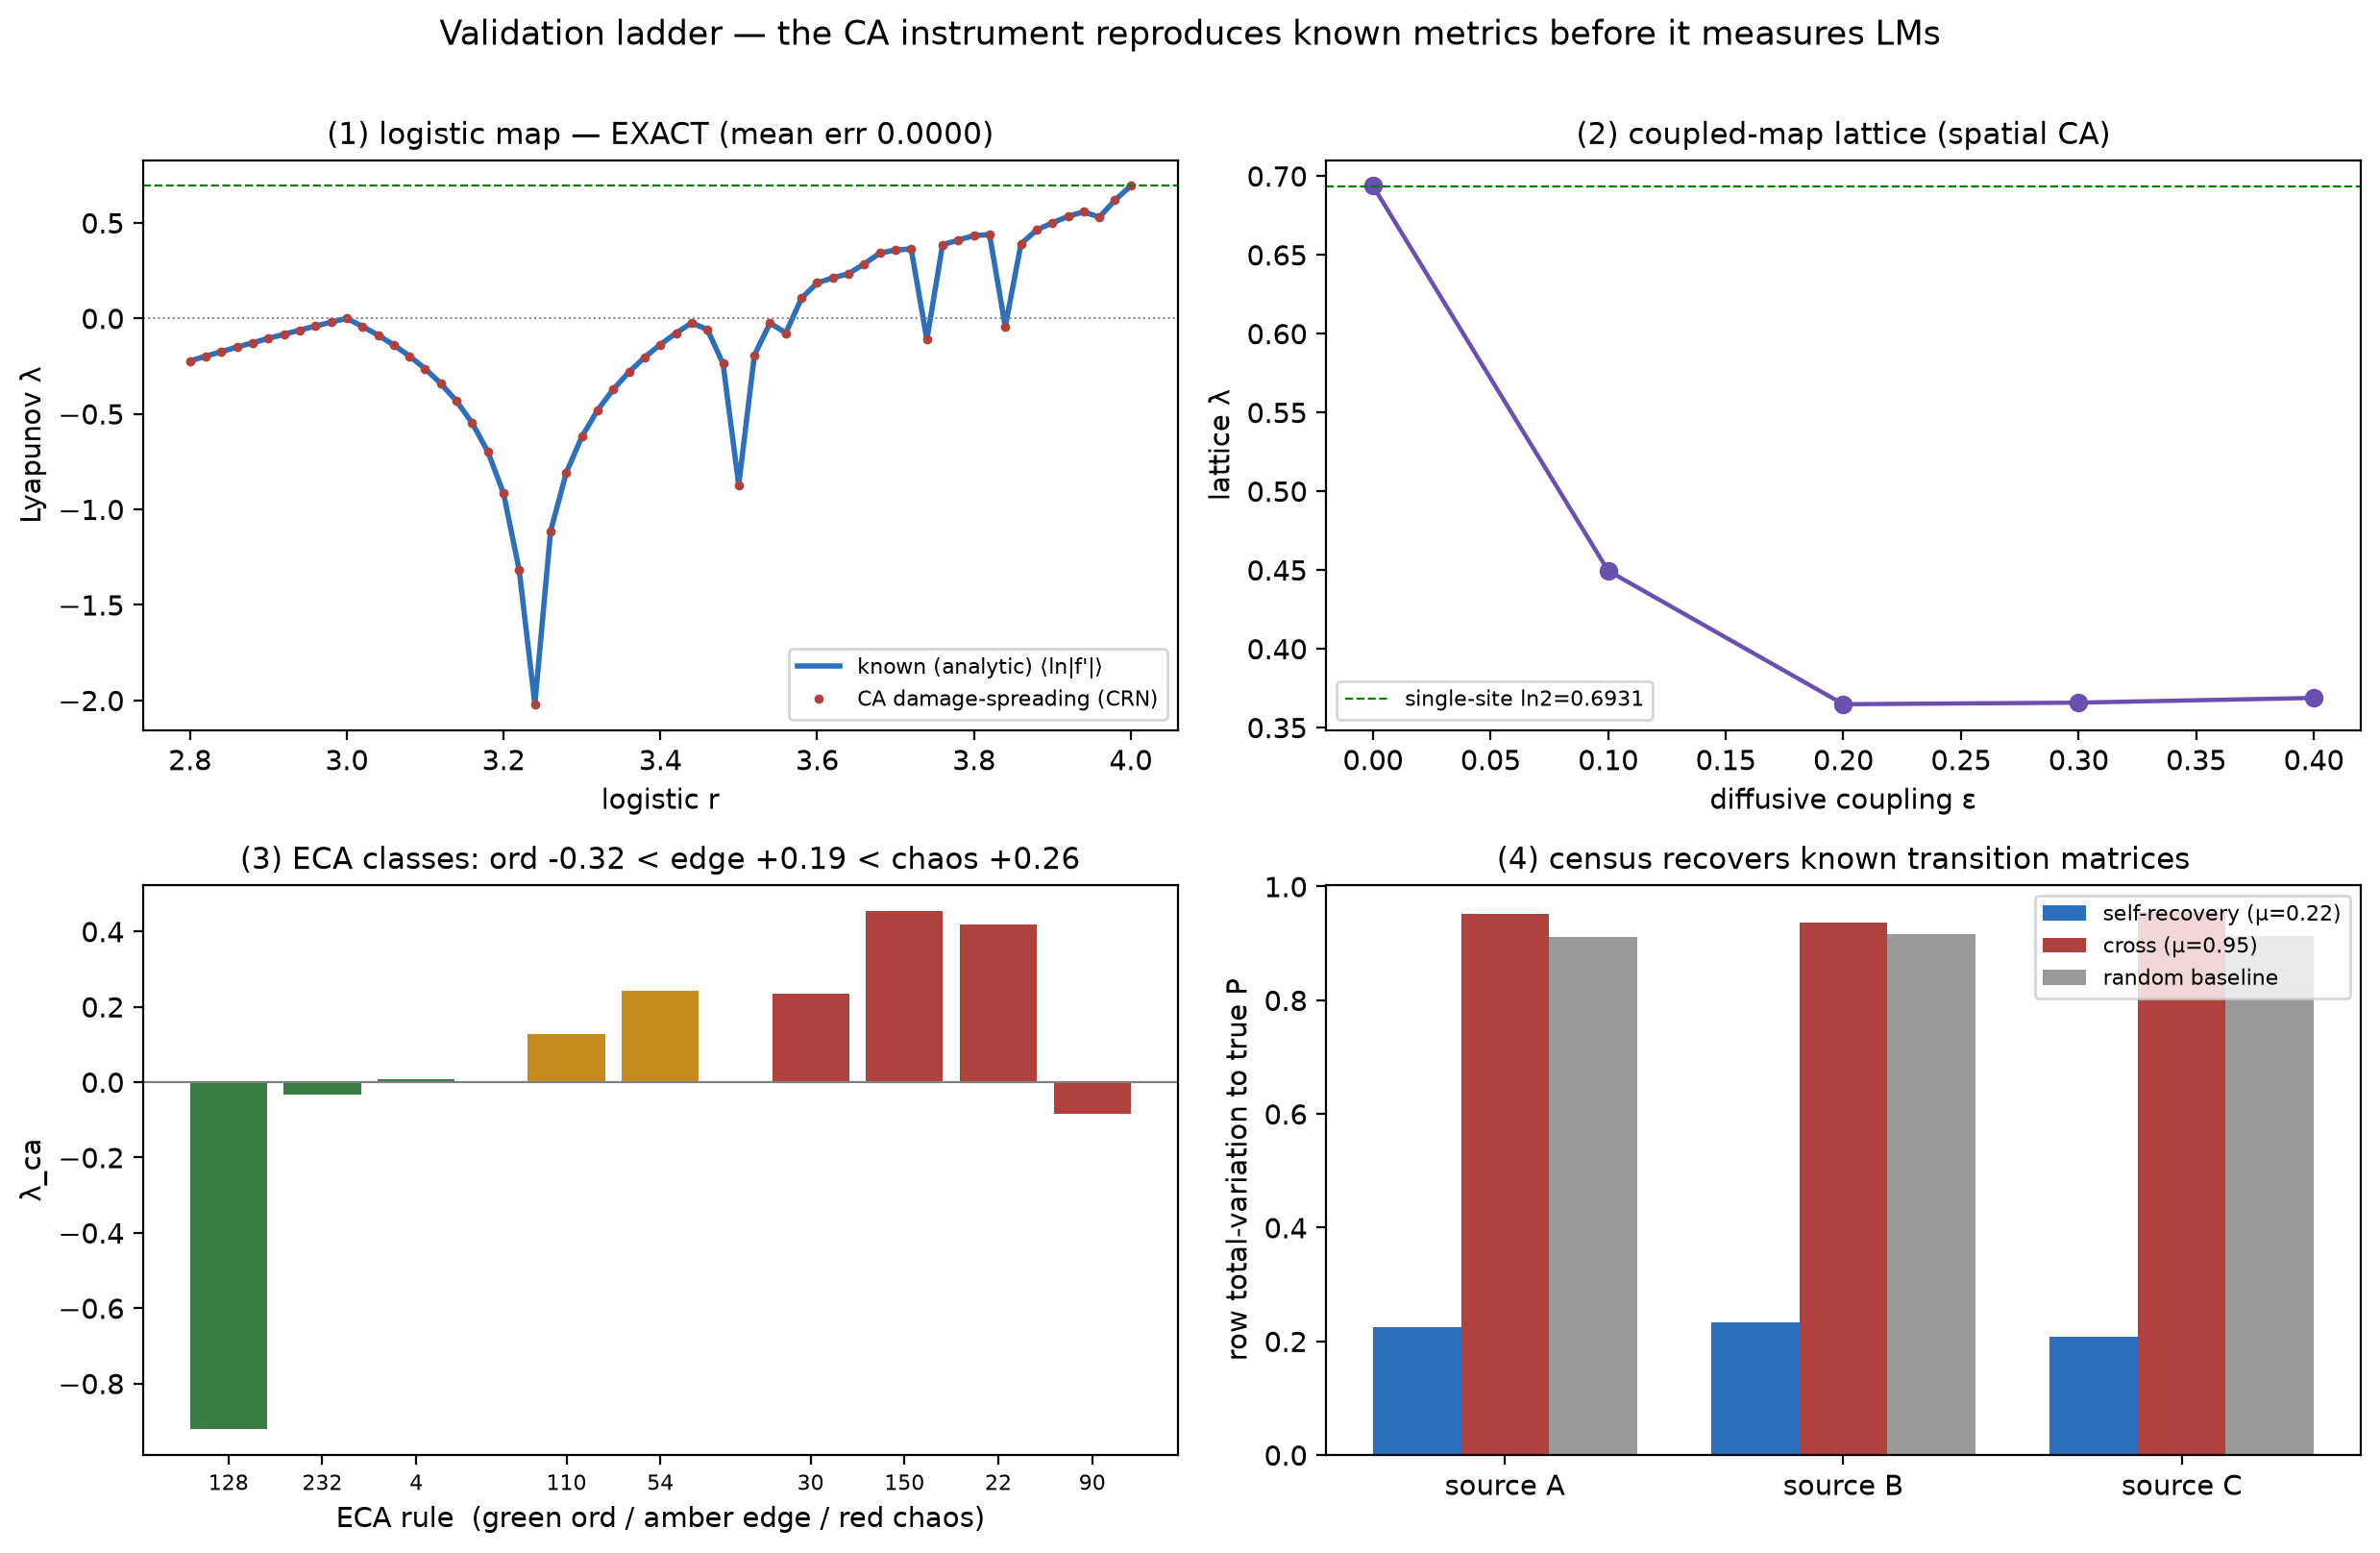
\includegraphics[width=0.97\linewidth]{validation_ladder.png}
\caption{Validation ladder, ordered by how much of the instrument's regime each rung shares;
only (3)--(5) are weight-bearing. Panel (4) is the load-bearing one: the DK damage field is
predicted by an independent simulator and matches cell-for-cell, with the off-line control
beside it showing the test is not vacuous.}\label{fig:ladder}
\end{figure}

\section{A developmental transition in token-space criticality}\label{sec:dev}
Applying the calibrated instrument across Pythia-410m training checkpoints
(\texttt{step256}--\texttt{step143000}, 8 seeds, two lattice sizes $N{=}48$ and $N{=}96$;
Fig.~\ref{fig:dev}) reveals a transition in the model's token-space dynamics. Early in
training the lattice is sub-critical for many seeds---a perturbation dies---and after the
transition it is super-critical for every seed, and remains so for the rest of training.

We pre-registered the test (post-transition vs.\ pre-transition checkpoints, run-level
Mann--Whitney, family $=\{\lca,\dn\}\times\{N{=}48,N{=}96\}$, Benjamini--Hochberg FDR) and a
demotion rule: failure at either lattice size demotes the headline. \textbf{All four members
survive} ($p_{\mathrm{BH}}\le2\times10^{-5}$). Measured from the pre-registered pre set
(steps $256/512$) to the settled plateau ($2000/8000/143000$), $\lca$ moves
$+0.0247\to+0.1683$ at $N{=}48$ ($d{=}1.59$, $p{=}5.9\times10^{-5}$) and
$+0.0197\to+0.1686$ at $N{=}96$ ($d{=}1.76$, $p{=}6.6\times10^{-5}$).

\textbf{The claim is better stated without any pre/post split at all}, since every effect
size depends on where that line is drawn. Before the transition the seeds do not agree on the
\emph{sign} of $\lca$ (6/16 negative at $N{=}48$, 8/16 at $N{=}96$, spanning $-0.216$ to
$+0.320$); after it, \textbf{not one of 48 plateau runs is negative}, the minimum being
$+0.107$. That uses all 96 runs and is what Fig.~\ref{fig:dev}C draws.

\textbf{The curve is not a step, and both ends of the contrast can be inflated.} It rises,
overshoots at step $1000$ by $1.4$--$22.4\%$, and settles. Taking the peak as the post value
inflates the effect; taking the lowest checkpoint alone as the pre value does the same at the
other end and by more ($1.7\times$ on $\lca$). We therefore use the pre-registered sets at
both ends. The overshoot survives correction in only one of four cells, and that cell is
\dn{}: on $\lca$---the quantity carrying the claim---it is $+14.3\%$ at $N{=}48$
($p_{\mathrm{BH}}{=}0.11$) and $+1.4\%$ at $N{=}96$ ($p_{\mathrm{BH}}{=}0.78$). So
non-monotonicity is largely a \dn{} phenomenon, and we do \emph{not} claim step $1000$ as a
distinct developmental phase.

\textbf{Which quantity carries the claim.} $\lca$ is size-robust: the effect does not shrink
with a doubled lattice ($104\%$ retention) and the plateau levels differ by $-0.0003$ with a
$95\%$ CI of $[-0.023,+0.022]$---they \textbf{agree to within $\pm14\%$}. We state this as a
bound rather than as a non-significant $p$-value, since a null result is not evidence of
equality. \dn{} is not size-robust: its gap roughly halves and its plateau level differs
decisively ($0.569$ vs.\ $0.306$, $p{=}1.3\times10^{-8}$), even though the standardized
effect is undiminished ($d$ $2.88\to3.07$)
because the variance shrinks too. So \dn{}'s \emph{discrimination} survives while its
\emph{absolute scale} does not. We therefore let $\lca$ carry the claim and report \dn{} as
same-direction corroboration at a stated lattice size, never as a lattice-free property.

\textbf{An unregistered observation, reported as one.} Seed-to-seed variance collapses across
the transition: $\mathrm{sd}(\lca)$ falls $0.136\to0.037$ at $N{=}48$ ($3.7\times$, Levene
$p{=}1.7\times10^{-4}$) and $0.124\to0.040$ at $N{=}96$ ($3.1\times$,
$p{=}7.7\times10^{-7}$). Before the transition, seeds disagree about the \emph{sign} of $\lca$;
after it every run is positive. They do not agree to a few percent---the plateau per-seed CV
is $22\%$ and $25\%$; the few-percent agreement is between lattice \emph{sizes}. Not
pre-registered, but it replicates independently at both sizes.

\begin{figure}[t]\centering
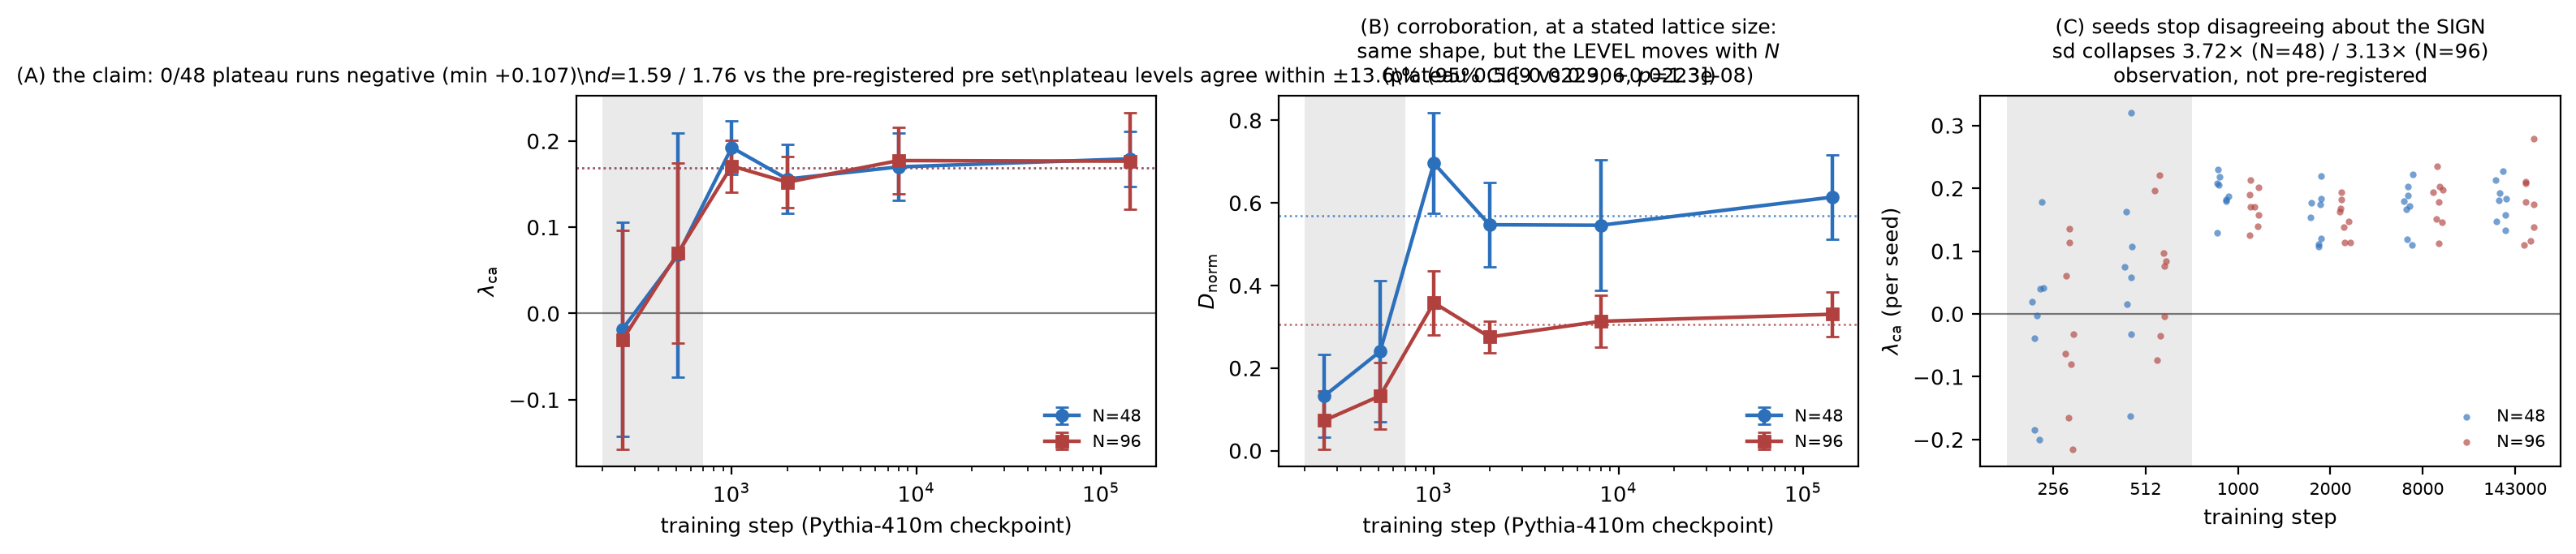
\includegraphics[width=0.97\linewidth]{developmental.png}
\caption{The developmental transition. (A) $\lca$ rises and settles positive; the two lattice
sizes lie on top of each other (plateau levels agree within $\pm14\%$). (B) \dn{} shows the same shape but
a size-dependent level---which is why it corroborates rather than carries. (C) Per-seed
values: sign disagreement before the transition, consensus after.}\label{fig:dev}
\end{figure}

\section{What the damping length measures: free generation absorbs nothing}\label{sec:realgen}
The instrument's central assumption---that a number measured on the ring says something about
the model---is one we tested rather than assumed, by running the identical damage protocol on
\emph{real autoregressive generation}. From a prompt we generate two CRN twins sharing one
uniform stream, force a different token at one position in one twin, and let both continue
freely; the null arm is asserted to diverge by exactly zero, and does.

The result is unambiguous and negative. On \texttt{pythia-70m}, \texttt{-160m} and
\texttt{-410m} (32 trials each) the injected error \textbf{persists in every single trial}
($P_{\text{persist}}{=}1.000$, $P_{\text{reconverge}}{=}0.000$). Token identity is a harsh
readout once an injection shifts alignment, so we also measured distributionally: the
total-variation distance between the twins' next-token distributions, normalized by the TV
between two \emph{independent} continuations of the same prompt, settles at
$\mathrm{TV_{norm}}\approx0.97$---the twins end as far apart as unrelated continuations.

The mechanism is structural, not a property of any model. \textbf{Free generation never
resamples a token}: once emitted, an error stays in context permanently. The ring CA revisits
every site, and in-place resampling is precisely what creates the possibility of healing. The
damping length, \dn{} and the light cone therefore characterise \emph{the iterated-resampling
construction}; they are not predictions about autoregressive decoding and we do not offer them
as such. This retroactively explains a light-cone velocity that depends on $r$ but not the
model, the model-invariance of $\lca(r)$, and the failure in \S\ref{sec:crosslevel}.

\textbf{What this does and does not cost.} It removes any reading of these quantities as
error-correction in deployed decoding. It does \emph{not} touch \S\ref{sec:dev}, and the reason
is worth stating: the construction is held \emph{fixed} across checkpoints---same ring, radius,
temperature, coupling, seeds---so a change measured across checkpoints cannot come from the
apparatus. A fixed instrument reading differently on different models is what an instrument is
for; what \S\ref{sec:realgen} forbids is transporting the reading's units to a process the
instrument does not implement.

\textbf{Coupling, stated precisely.} Damage spreading is a property of \emph{(model,
coupling)}, not of the model alone---a published result in stochastic PCAs, where the damage
boundary moves with the replica-coupling algorithm while single-replica dynamics is insensitive
to it \citep{kohring1992,grassberger1995}. Our inverse-CDF sampling from a shared uniform is
the \emph{monotone} coupling: on DK's binary alphabet it coincides with the maximal-correlation
member of the admissible family \citep{hinrichsen1997}, which is why the identity above is
exact, but on a vocabulary it does not, so our LM damage numbers sit inside the family rather
than at an extremum (measured excess disagreement $1.3$--$5.4\%$; see the repository). The
property that justifies the choice is replica-independence---each replica's next state depends
on its own state and the shared noise alone---which a pairwise maximal coupling lacks.
Relative comparisons, including \S\ref{sec:dev}, are unaffected: the coupling is a common mode.

\section{Other readings, briefly}\label{sec:other}
Two further quantities, reported compactly because \S\ref{sec:realgen} bounds what they mean.
\emph{Effective interaction radius}: under the repetition-robust metric, long-range corpus
consistency peaks at $r\approx4$ and falls by $r{=}16$---the apparent large-$r$ growth is
collapse into repetition. Cross-model profiles exceed the apparatus floor at a fixed windowing
scheme, but the scheme moves the profile as much as a model change does. \emph{Damage light
cone}: a block flip produces a ballistic front whose velocity grows monotonically with $r$ and
is \textbf{model-invariant} (apparent plateaus on small rings are wraparound, $v\approx N/4$).
This is the classic CA light cone \citep{bagnoli1992damage,lieb1972finite,butterfly_ca}; we
show the token lattice exhibits it and do not claim the law as new. Both constructions
replicate the radius-level measurements, evidence they are not tied to masked windowing.

\section{The instrument's boundary: token- vs.\ activation-space}\label{sec:crosslevel}
A black-box instrument earns its keep if its readings track something one would otherwise need
internals to see. We tested this thoroughly---calibration, two model families, two within-model
axes---and report a clean \textbf{negative}. Pairing the token-space reading against a
finite-depth top-Lyapunov exponent of the residual stream is family-dependent (Pythia
$r{=}{+}0.71$, GPT-2 $r{=}{-}0.43$; the pooled $p{=}0.025$ is a Simpson's-paradox artifact).
Within-model, the temperature axis is confounded by a common cause and the radius axis is null,
because $\lca(r)$ is model-invariant and so carries no model signal to proxy. The reason is
structural: the white-box exponent is \emph{architectural}---flat across training and
$\approx1/L$---so a masked-family correlation with depth is depth-mediated. A regime mismatch
compounds it: that exponent is a \emph{tangent} quantity while $\lca$ is a \emph{finite} one,
and our own $\epsilon$-sweep shows the two disagree even where ground truth is known.
Token-space and activation-space criticality are distinct, non-proxying levels.

\section{Related work}
\textbf{The framing is not our claim.} Iterated-LLM views exist qualitatively
\citep{logos_ca,telephone,paraphrase2cycle} and rigorously for masked-LM Glauber dynamics
\citep{glauber_mlm}; our novelty is the measurement layer, not the framing. \textbf{Edge of
chaos.} Canonical \citep{langton1990computation,bertschinger2004real}, and already applied to
trained transformers via self-attention Jacobians \citep{lyap_selfattn} and to LLMs generally
\citep{edgeofchaos2024,qle}; we claim neither the concept nor the
criticality$\leftrightarrow$capability link. \textbf{Critical sampling temperature} is defined
and measured in at least five prior works
\citep{critical_temp,critical_temp2,critical_temp3,ar_tempcrit,phase_detect}; we claim only a
calibrated route to it, not the quantity. \textbf{Perturbation propagation} in
\emph{activation} space \citep{sparc,tft,residual_dynamics} and over compound-AI graphs
\citep{quiver} is adjacent but in a different space. \textbf{Terminology}: we avoid ``repair''
\citep{hydra,selfrepair} and ``self-correction'' \citep{sparc}, both categorically different
from a spatial damping length. \citet{sampler_oracle} is the calibration kin; the census
descends from \citet{hanson1997computational}.

\section{Limitations}
Masked-LM conditionals are globally inconsistent and the autoregressive rule, though
consistent, is resampled in place on a ring: neither construction samples the model's actual
distribution, so all claims are properties of the dynamics. Rings are small ($N\le384$) and
the developmental result rests on one model family at two lattice sizes; a third size and a
second family are the obvious next requirement. \dn{}'s absolute scale is doubly
qualified---it moves with $N$ (\S\ref{sec:dev}) and its numerator's coupling is not extremal
(\S\ref{sec:realgen})---so only its relative behaviour is quoted. Census ground truth is
synthetic only; on real models it is proxy-scored and near-floor. The windowing scheme is a
first-class apparatus factor, and temperatures are not comparable across constructions.
\textbf{Statistical scope.} The developmental family is pre-registered with BH-FDR at the run
level; the ECA test uses the rule as the unit. The ladder reproductions are exact or
near-exact matches to known values and do not rest on hypothesis testing. The cross-level
negative rests on sign-consistency across families and axes, not a surviving $p$-value. A
previously reported capacity$\to$sensitivity axis was pseudoreplicated and is retracted.

\section{Conclusion}\label{sec:conclusion}
The contribution is a \emph{validated} black-box instrument and an honest account of its
range. Before measuring a model, the apparatus reproduces a stochastic PCA's damage spreading
bit-exactly, separates CA rules by whether damage survives, and recovers known transition
matrices. Pointed at Pythia checkpoints it detects a developmental transition in token-space
criticality that survives pre-registered correction at two lattice sizes. Pointed at real
generation it returns a negative that bounds all of it: free generation absorbs no injected
token error, so these measure an iterated-resampling construction. An instrument that recovers
what is known, says which of its checks are load-bearing, and marks where its readings stop
applying is more useful than one that claims more.

\bibliographystyle{plainnat}
\bibliography{refs}

\appendix
\section{Reproducibility}
\textbf{Models.} \texttt{bert-tiny}/\texttt{mini}/\texttt{base} ($L{=}2$--$24$);
\texttt{Pythia-14M}--\texttt{1B} \citep{pythia} and \texttt{GPT-2} small--xl; Pythia-410m
checkpoints \texttt{step256}--\texttt{step143000}. A tiny transformer trained from scratch on
tinyshakespeare provides the corpus-checked census. \textbf{Grids.} $r\in\{1,2,4,8,16\}$,
$T\in\{0.3,\dots,1.5\}$, $N\in\{48,96,192,384\}$, 8 seeds for the developmental family.
\textbf{Definitions.} $\dn=D/\dz$ with \dz{} the independent-noise no-flip floor; \lca{} the
log-slope of damaged-site count over the pre-saturation window, with the fit window's
constants exposed as parameters and a named sentinel for never-ignited runs. \textbf{Tests.}
The exact-zero CRN null is asserted over every backend and both update modes through one
shared simulation loop; a golden-file regression asserts the core stays bit-identical; the DK
identity is asserted cell-for-cell with an off-line control that must fail. All code,
per-run result files, and figure scripts accompany the submission; every number in the paper
is traceable to a result file.

% NeurIPS Paper Checklist — \input this at the end of the NeurIPS-formatted paper
% (after \bibliography, before \end{document}). Answers are honest to the current
% state; update the [TODO] items before submission.
\newpage
\section*{NeurIPS Paper Checklist}

\begin{enumerate}
\item {\bf Claims} \\
Question: Do the abstract and introduction accurately reflect the paper's contributions and scope? \\
Answer: \answerYes{} \\
Justification: The abstract states the contribution as the instrument and its measurements, explicitly frames the criticality/edge-of-chaos phenomena as decades-old (measured, not discovered), and flags that the capacity effect is masked-specific and does not replicate on autoregressive models. Every headline claim is hedged to its statistics: the capacity ordering is presented as a suggestive two-seed gap (tiny$\ll$\{mini,base\}), not an established scaling axis; the front velocity as an apparatus-kinematic law; the AR capacity trend as a null. A withdrawn kinematics$\perp$stability decomposition is disclosed rather than retained.

\item {\bf Limitations} \\
Question: Does the paper discuss the limitations of the work? \\
Answer: \answerYes{} \\
Justification: The Limitations section states: globally-inconsistent MLM conditionals (a well-defined dynamical system but not a sampler of any joint); small models ($\le$110M masked, $\le$1B AR) and small rings ($N\le384$); proxy census (WikiText, not the models' training data); the AR capacity trend rests on few models; the special-token scheme is a first-class apparatus; temperature scales are not comparable across constructions.

\item {\bf Theory assumptions and proofs} \\
Question: For each theoretical result, does the paper provide the full set of assumptions and a complete (and correct) proof? \\
Answer: \answerNA{} \\
Justification: The paper contains no formal theorems; it is empirical/measurement work. Connections to the Lieb--Robinson bound and the Bagnoli--Rechtman--Ruffo Lyapunov--velocity relation are cited, not re-derived.

\item {\bf Experimental result reproducibility} \\
Question: Does the paper fully disclose all the information needed to reproduce the main experimental results? \\
Answer: \answerYes{} \\
Justification: All code, model checkpoints (toy), per-run result JSON/NPZ, and figures are in the public repository; the Reproducibility appendix gives models, grids, seeds, batch/ring sizes, the diversity-floor and CRN definitions, and the statistical tests. A harness regression test asserts the CRN null coupling is exactly zero.

\item {\bf Open access to data and code} \\
Question: Does the paper provide open access to the data and code, with sufficient instructions? \\
Answer: \answerYes{} \\
Justification: Repository with a README giving per-phase reproduction commands and M1 runtime tables; pinned dependency versions; scripts are idempotent and resumable. [TODO: make the repository public and add the URL at camera-ready.]

\item {\bf Experimental setting/details} \\
Question: Does the paper specify all the training and test details? \\
Answer: \answerYes{} \\
Justification: Reproducibility appendix specifies optimizer/steps for the toy model, the exact $(r,T,N,B,\text{sweeps},\text{seeds})$ grids per experiment, the reference corpora, and the metric definitions.

\item {\bf Experiment statistical significance} \\
Question: Does the paper report error bars / statistical significance? \\
Answer: \answerYes{} \\
Justification: The paper reports seed error bars and trend tests and, following an internal adversarial audit, explicitly \emph{retracts} a pseudoreplicated signed-rank statistic on the capacity claim, restating it as a suggestive two-seed gap (tiny$\ll$\{mini,base\}; base-vs-mini null $p=0.21$; AR size trend Spearman $\rho=0.17$, $p=0.29$). Marginal and null results are labeled as such. [TODO: the tracked pre-camera-ready rebuild raises the headline capacity/damping-length claims to $\ge15$ \emph{independent} seeds with a seed-level (hierarchical/bootstrap) test and a multiplicity correction; see repository issues \#1--\#3, \#9.]

\item {\bf Experiments compute resources} \\
Question: Does the paper provide sufficient information on compute resources? \\
Answer: \answerYes{} \\
Justification: All experiments run on a single Apple M1 Pro (16\,GB); per-phase wall-clock runtimes are tabulated. The toy model uses CPU JAX; real models use fp16 on the MPS backend. Total compute is a few laptop-days.

\item {\bf Code of ethics} \\
Question: Does the research conform with the NeurIPS Code of Ethics? \\
Answer: \answerYes{} \\
Justification: Measurement/interpretability work on public pretrained models and synthetic data; no human subjects, no sensitive data, no new capability that raises misuse concerns.

\item {\bf Broader impacts} \\
Question: Does the paper discuss potential positive and negative societal impacts? \\
Answer: \answerYes{} \\
Justification: The instrument is a black-box interpretability tool (positive: measurement of trained-LM token dynamics without weight access, applicable to closed models). It creates no new generative capability; negative societal impact is minimal and indirect. [TODO: one broader-impacts paragraph.]

\item {\bf Safeguards} \\
Question: Does the paper describe safeguards for responsible release of high-risk assets? \\
Answer: \answerNA{} \\
Justification: No high-risk models or datasets are released; only measurement code and analysis results on public models.

\item {\bf Licenses for existing assets} \\
Question: Are existing assets (code, data, models) properly credited and licenses respected? \\
Answer: \answerYes{} \\
Justification: Pretrained models (BERT, Pythia), datasets (tinyshakespeare, WikiText-103), and libraries (JAX, PyTorch/Transformers) are cited; usage is within their licenses. [TODO: list exact licenses in the appendix at camera-ready.]

\item {\bf New assets} \\
Question: Are new assets introduced in the paper well documented? \\
Answer: \answerYes{} \\
Justification: The instrument (code), the synthetic-Markov calibration corpora, and the toy checkpoints are documented in the repository README and the Reproducibility appendix.

\item {\bf Crowdsourcing and research with human subjects} \\
Question: N/A. \\
Answer: \answerNA{} \\
Justification: No human subjects or crowdsourcing.

\item {\bf Institutional review board (IRB) approvals} \\
Answer: \answerNA{} \\
Justification: No human-subjects research.

\item {\bf Declaration of LLM usage} \\
Question: Does the paper describe LLM usage if it was an important, original, or non-standard component? \\
Answer: \answerYes{} \\
Justification: Pretrained LLMs are the object of study (the CA rule), documented throughout. [TODO: disclose any LLM assistance in writing/experimentation per venue policy.]
\end{enumerate}


\end{document}
